\documentclass[
  manuscript=article,  
  layout=preprint,  
]{format}

\usepackage{soul}
\usepackage{gensymb}

% --- blew is the area for authors ---

\usepackage[english]{babel}
\usepackage{comment}

% specify the .bib file for references
\addbibresource{reference.bib} 

% Make sure your article tile is within 12 words
\title{Influencia de la heterogeneidad espacial en la evaluación de la susceptibilidad por movimientos en masa}

\author{Edier Aristizábal}
\affiliation{Departamento de Geociencias y Medio Ambiente, Universidad Nacional de Colombia, Medellín, Colombia}

% maximum five keywords
\keywords{landslide; susceptibility; spatial heterogeneity} 

\begin{document}

\begin{abstract}
This study explores the incorporation of spatial heterogeneity in modeling landslide susceptibility in the complex terrain of the Colombian Andes. The data used included a dataset of 13,777 landslides recorded between 1970 and 2023, derived from high-resolution optical imagery, as well as precipitation data from the CHIRPS dataset. Additional spatial information, such as land cover, was derived using Sentinel-2 data processed in Google Earth Engine. These diverse geospatial data sources were integrated to provide a comprehensive understanding of the factors influencing landslide susceptibility. By applying Geographically Weighted Regression (GWR) and its extension, Multiband Geographically Weighted Regression (MGWR), we demonstrate significant improvements in the capacity of models to capture local variability and enhance predictive accuracy. GWR and MGWR allow for the identification of spatially differentiated patterns and specific scales of influence for each predictor, leading to a more precise representation of landslide susceptibility and highlighting the necessity of adapting models to the unique geographic context of each region. However, the study also underscores the need for careful bandwidth selection to avoid overfitting and ensure model stability. Despite the advantages of GWR and MGWR, limitations such as high computational complexity and local collinearity were identified, which can impact the interpretation and reliability of the results.
\end{abstract}

\section{Introducción}
En las últimas décadas, el empleo de modelos estadísticos o de aprendizaje de máquinas (\textit{machine learning}) han tenido una relevancia creciente en la evaluación de la susceptibilidad a movimientos en masa (\cite{aristizabal2015susceptibility, tehrani2022machine, korup2014landslide}). Estos enfoques metodológicos se han consolidado como herramientas muy útiles para construir mapas de susceptibilidad, permitiendo identificar zonas más propensas por sus condiciones naturales a experimentar movimientos en masa. Los mapas de susceptibilidad por movimientos en masa son utilizados para el ordenamiento territorial, estudios ambientales, así como para la gestión del riesgo de desastres, entre otros (\cite{guzzetti1999landslide, soeters1996, corominas2014recommendations}).

Los modelos estadísticos expresan la correlación entre una variable respuesta (también denominada variable dependiente, resultado o de salida) y un conjunto de variables predictoras (covariables, variables independientes o regresores) (\cite{dai2001assessment}). Estos métodos suponen que las condiciones geológicas, topográficas y climáticas que llevaron a la ocurrencia de movimientos en masa en el pasado proporcionan la información necesaria para establecer las ubicaciones y condiciones de futuros movimientos en masa sobre las laderas. Por lo que exigen contar con un inventario de movimientos en masa (\cite{dai2001assessment, brabb1984innovative, soeters1996}). 

Una de las principales limitaciones de los modelos tradicionales para la evaluación de la susceptibilidad a movimientos en masa es la suposición de homogeneidad espacial (\cite{lombardo2020space}). Los coeficientes que entregan estos modelos representan una valor medio. Es decir, estos modelos asumen que la influencia de las variables predictoras con la variable respuesta es constante en todo el área de estudio, implicando que el terreno se considera homogéneo en términos de su respuesta a los movimientos en masa.  Esta simplificación permite un modelado más sencillo, pero no captura la complejidad inherente a los sistemas naturales, donde la distribución espacial e influencia de los factores condicionantes en la ocurrencia de movimientos en masa, como la geología, las formas del terreno, el clima o la vegetación, pueden variar de manera significativa.

La heterogeneidad espacial es una característica fundamental de los datos geoespaciales y suponen importantes desafíos para los modelos estadísticos convencionales (\cite{anselin1988spatial, cressie2015statistics, lesage2009introduction}). La heterogeneidad espacial se refiere a la variabilidad de las condiciones del terreno a lo largo del espacio (\cite{anselin1990spatial}). Por ejemplo, las propiedades geomorfológicas de una ladera pueden diferir sustancialmente de las de otra dentro de una misma cuenca, afectando la susceptibilidad de cada zona a los movimientos en masa.  Ignorar esta heterogeneidad del espacio puede llevar a una subestimación o sobrestimación de la susceptibilidad en ciertas zonas del área de estudio.

Para abordar estas limitaciones, se han desarrollado modelos que permiten la variación espacial de los coeficientes de las variables predictoras, permitiendo capturar la heterogeneidad inherente al terreno (\cite{rey2023geographic}). Entre estos enfoques se encuentran los modelos multiniveles (\cite{wong1985hierarchical}) (también conocidos como jerárquicos, y en algunos casos modelos mixtos o regímenes espaciales) y los modelos de regresión espacial ponderada (GWR, por sus siglas en inglés) (\cite{brunsdon1996geographically}). Los modelos multiniveles permiten modelar la variabilidad espacial mediante la introducción de estructuras jerárquicas, asignando un coeficiente e intercepto para cada nivel o región incorporada en el modelo. Lo cual resulta particularmente útil cuando los datos presentan una organización natural en grupos o niveles (por ejemplo, cuencas y subcuencas). En contraste, los modelos GWR son menos complejos computacionalmente, ya que no requieren definir niveles jerárquicos. Los modelos GWR permiten que los coeficientes de las variables predictoras varíen para cada observación, proporcionando una caracterización más detallada de la influencia de las variables en función de su localización geográfica. Ambos enfoques presentan ventajas significativas frente a los modelos tradicionales, al capturar la variabilidad espacial, mejorando la precisión en la evaluación de la susceptibilidad a movimientos en masa.

En este trabajo, se explora la influencia de la heterogeneidad espacial en a evaluación de la susceptibilidad por movimientos en masa. Para ello, se utilizan cuencas hidrográficas como unidades de mapeo, una elección que permite ajustarse de manera más adecuada a las condiciones naturales del territorio. Además, en lugar de emplear una variable dependiente binaria, se utilizó la frecuencia de movimientos en masa, lo cual proporciona una mejor comprensión del fenómeno y permite explorar la variabilidad espacial de la influencia de las variables predictoras en el área de estudio. El objetivo principal de este trabajo no se encuentra tanto en la producción de un mapa de susceptibilidad, sino en evaluar la heterogeneidad espacial de las covariables y su influencia en la evaluación de la susceptibilidad por movimientos en masa. Este enfoque pretende aportar en la comprensión  de la heterogeneidad espacial de los factores condicionantes, lo cual es crucial para la implementación de modelos de susceptibilidad que logren capturar de forma adecuada el fenómeno en cuestión.

\section{Modelo de regresión espacial ponderada}

Los Modelos de Regresión Espacial Ponderados (GWR, por sus siglas en inglés) constituyen una herramienta estadística avanzada desarrollada para analizar la heterogeneidad espacial de relaciones entre una variable respuesta y un conjunto de variables predictoras en un contexto geográfico (\cite{brunsdon1996geographically, fotheringham2000quantitative, fotheringham2009geographically}). A diferencia de los modelos de regresión tradicional, que asumen que la relación entre las variables es constante en todo el espacio de estudio, los modelos GWR permiten que los coeficientes varíen de manera local. Esto se logra ajustando un modelo de regresión independiente en cada ubicación geográfica, utilizando datos cercanos para ponderar las estimaciones (\cite{brunsdon1996geographically}). Esta metodología es particularmente valiosa para el análisis de susceptibilidad a movimientos en masa, ya que permite representar cómo las diferentes condiciones del terreno afectan la susceptibilidad de manera no uniforme a lo largo de un área.

La formulación matemática de un modelo de regresión espacial ponderada es de la siguiente forma (\cite{brunsdon1996geographically}):

\[
y_i = \beta_0(u_i, v_i) + \sum_{k=1}^p \beta_k(u_i, v_i) x_{ik} + \epsilon_i
\]

donde: \( y_i \) es el valor de la variable respuesta en la ubicación \( i \), \( (u_i, v_i) \) las coordenadas geográficas de la ubicación \( i \), \( \beta_0(u_i, v_i) \) el término independiente local en la ubicación \( i \), \( \beta_k(u_i, v_i) \) el coeficiente local asociado con la variable predictora \( x_{ik} \) en la ubicación \( i \). \( x_{ik} \) es el valor de la variable predictora \( k \) para la ubicación \( i \), y \( \epsilon_i \) el término de error en la ubicación \( i \).

Los modelos GWR son útiles en situaciones donde la influencia de las variables predictoras cambia espacialmente (\cite{fotheringham2009geographically}), es decir. En estudios de movimientos en masa, estas relaciones pueden depender de la topografía local, las características del suelo, la vegetación, o incluso de los patrones de precipitación que varían en el espacio. Por ejemplo, la influencia de la pendiente o la cobertura vegetal sobre la susceptibilidad a movimientos en masa puede ser distinta en regiones con diferentes características geológicas o climáticas. La aplicación de GWR permite capturar esta variabilidad y proporciona un análisis más detallado y específico para cada localidad del área de estudio.

El aspecto clave de la GWR es que los coeficientes  varían dependiendo de la ubicación geográfica , lo cual se logra a través del uso de un kernel de ponderación que da más peso a las observaciones cercanas y menos peso a las observaciones lejanas (\cite{fotheringham2000quantitative}). En la práctica, este kernel suele ser una función gaussiana o una función adaptativa, que ajusta el peso según la distancia desde el punto central.

Una de las principales ventajas de los modelos GWR es la facilidad con la que los resultados de GWR pueden ser interpretados y visualizados en un contexto espacial, facilitando la identificación de patrones locales de susceptibilidad y ayudando a la toma de decisiones. Los mapas de coeficientes permiten identificar áreas donde ciertas variables tienen una mayor o menor influencia, aportando información útil para el manejo territorial y la planificación.

Sin embargo, los modelos GWR también presentan limitaciones importantes. Una de ellas es la multicolinealidad local, ya que, debido a la naturaleza local de las regresiones, es posible que en algunas áreas las variables predictoras estén altamente correlacionadas, lo que dificulta la interpretación de los coeficientes (\cite{fotheringham2000quantitative, brunsdon1996geographically}). Además, los modelos GWR suelen ser computacionalmente más exigentes que los modelos de regresión globales o clásicos, especialmente cuando se trabaja con grandes volúmenes de datos espaciales.

Otra limitación a destacar es la selección del ancho de banda (BW) del kernel de ponderación (\cite{guo2008comparison}). El BW determina cuántas observaciones se consideran en el cálculo de los coeficientes locales, y su elección tiene un impacto en los resultados del modelo. Un BW demasiado amplio puede resultar en un modelo más similar a una regresión global, mientras que un BW muy estrecho puede llevar a resultados sobre-ajustados y poco generalizables. La selección adecuada del BW suele requerir un proceso iterativo y cuidadoso.

\section{Área de estudio y datos}

\par El área de estudio se localiza al norte del paralelo 5$^{\circ}$N y tiene una extensión aproximada de 50,000 km$^2$ (Fig. \ref{fig:localizacion}). Incluye las Cordilleras Occidental y Central de los Andes colombianos, las cuales se encuentran separadas por el cañón del río Cauca, una prominente depresión geográfica. Los límites naturales del área de estudio están definidos por el río Magdalena al este y el río Atrato al oeste. Dentro de este territorio se han delimitado 533 microcuencas. Aproximadamente el 73\% de estas microcuencas tienen una extensión menor a 100 km$^2$, con un área promedio de 48 km$^2$. Esta configuración hidrográfica refleja la compleja interacción entre procesos geomorfológicos y las variadas condiciones topográficas y climáticas que caracterizan a los Andes colombianos.

\begin{figure}[ht!]
    \centering
      {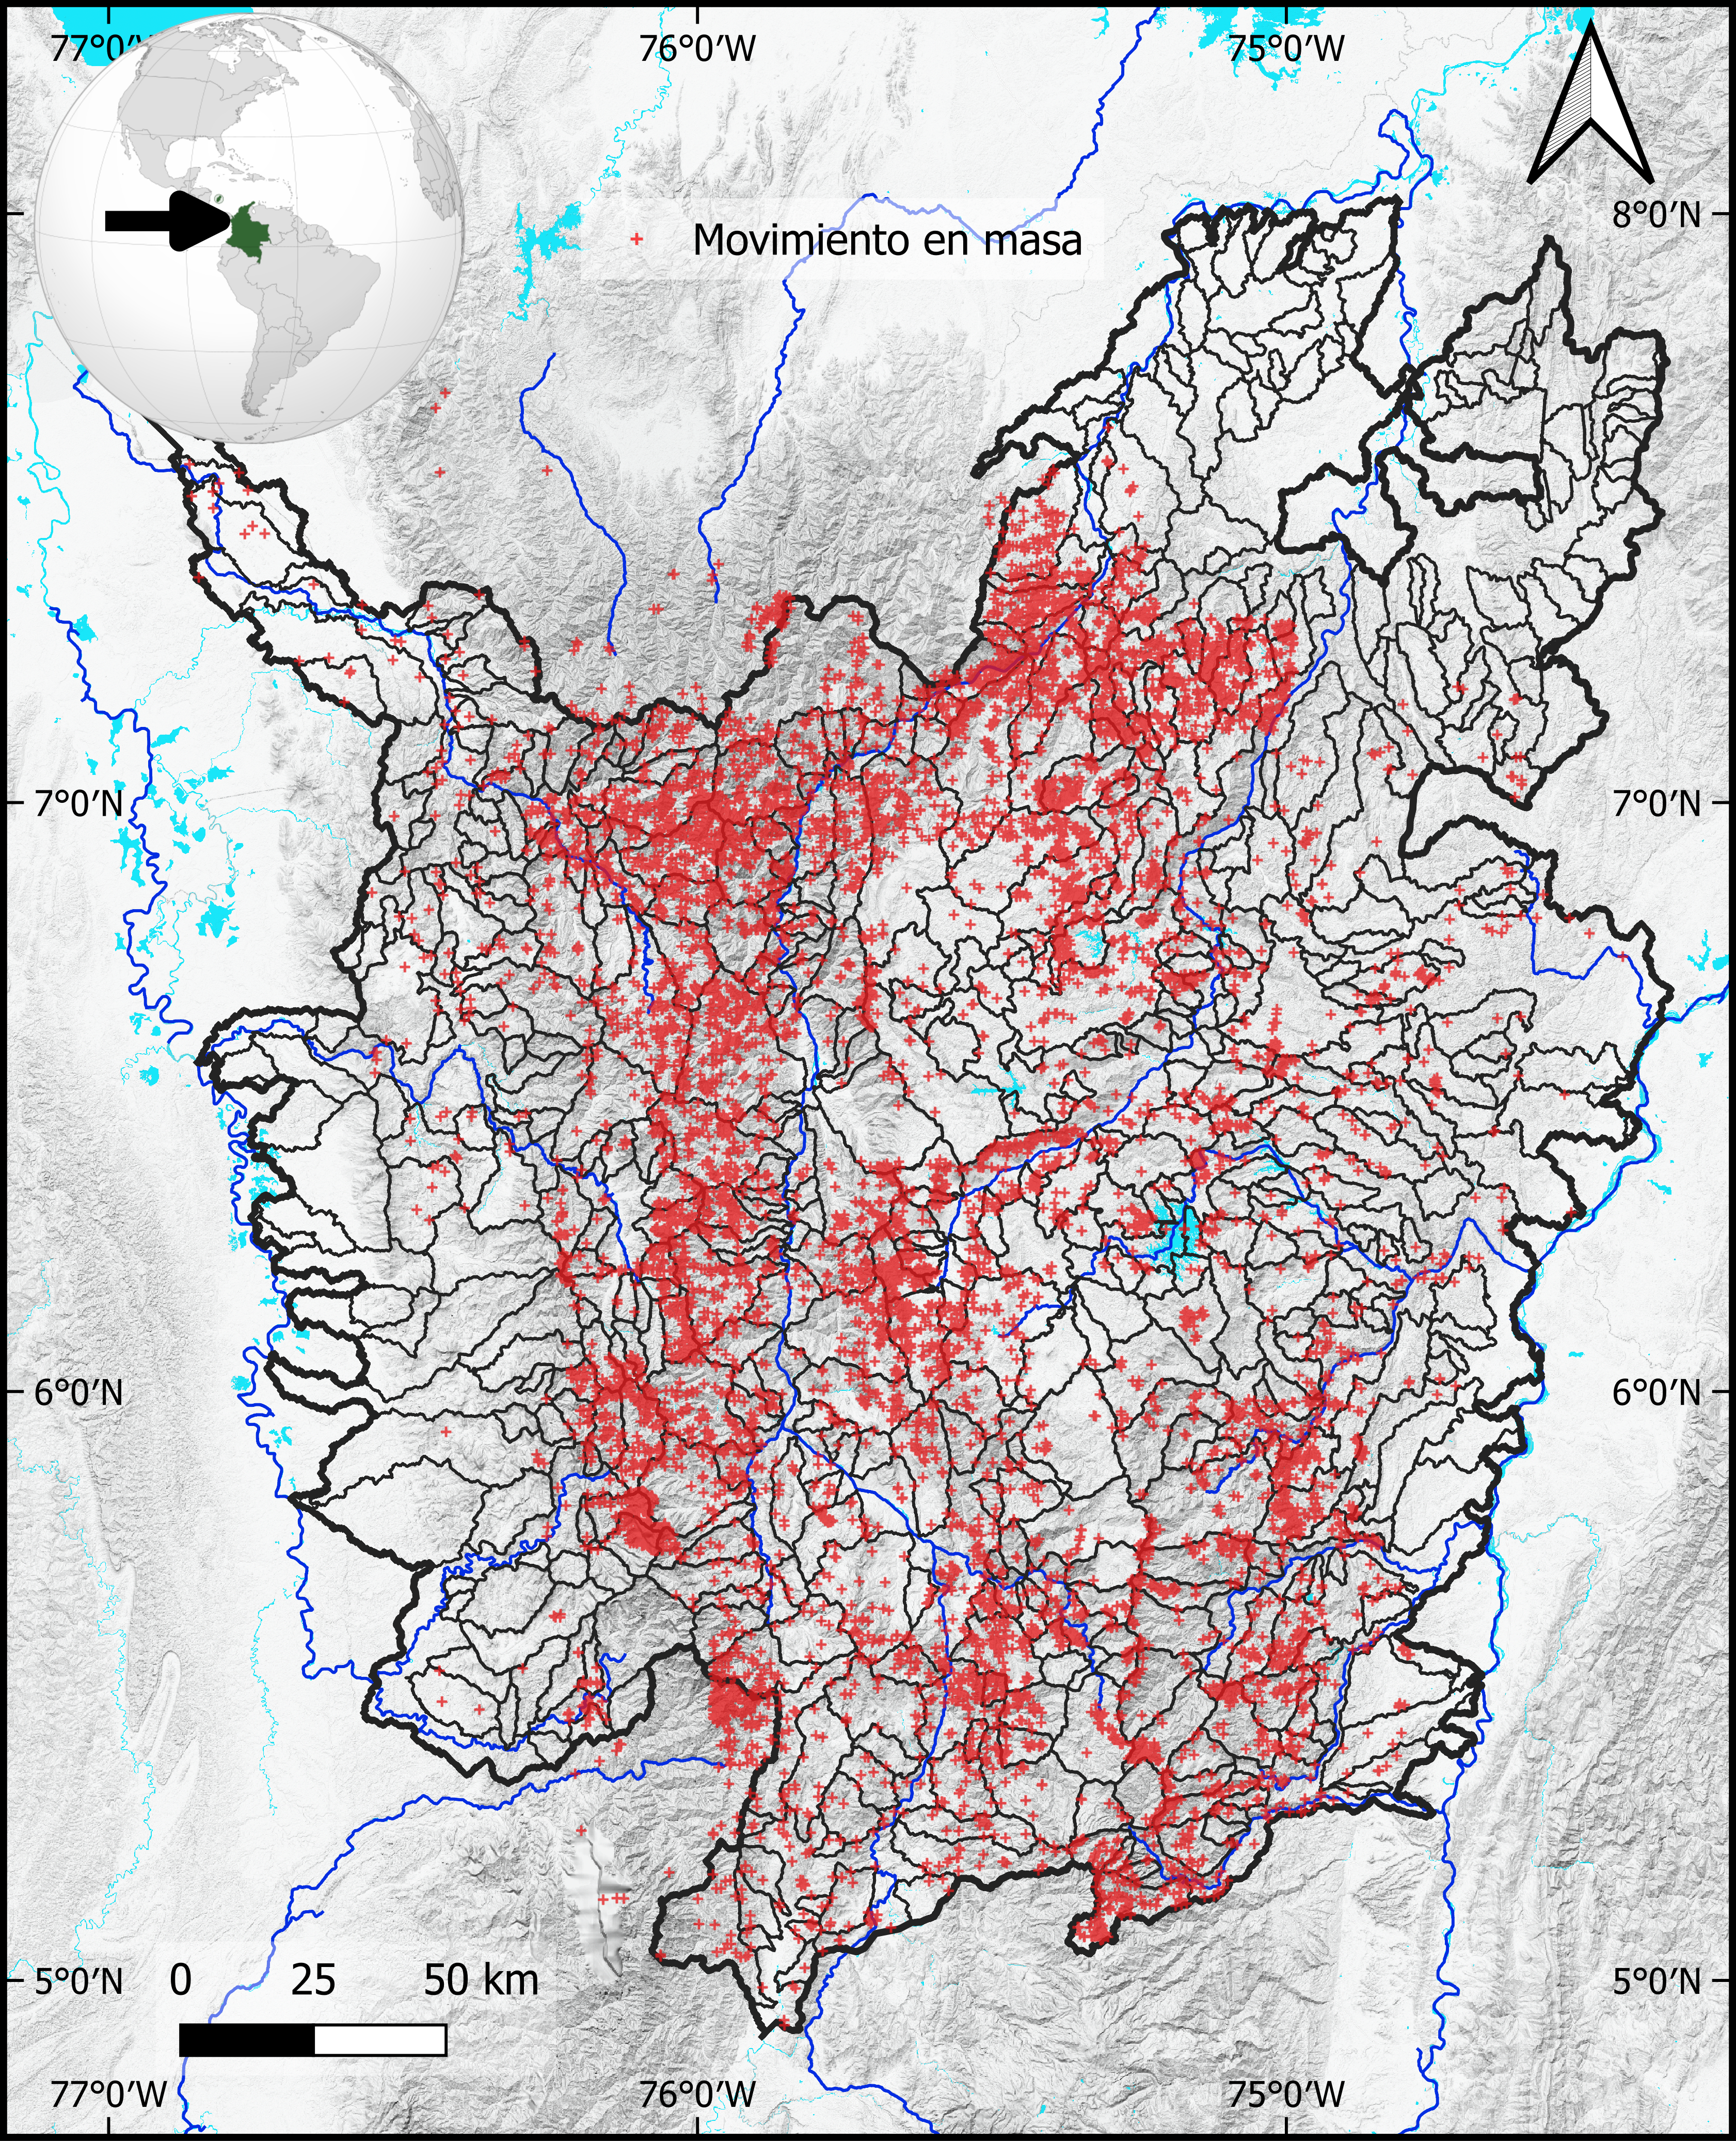
\includegraphics[width=0.8\textwidth]{figures/localizacion.png}}
\caption{Mapa de localización del área de estudio en las Cordilleras Occidental y Central de los Andes colombianos. Los puntos rojos representan los movimientos en masa registrados entre 1970 y 2023. Se muestran los principales ríos y la delimitación de las 533 subcuencas. }
    \label{fig:localizacion}
\end{figure}

\par Las variables predictoras seleccionadas para el área de estudio comprenden distintos aspectos geomorfológicos, climáticos y geológicos. Estas incluyen el área bajo la curva hipsométrica de cada microcuenca, elevación media, relieve local medio y precipitación media anual. Estas variables fueron seleccionadas en base a su relevancia para los procesos de inestabilidad de laderas, proporcionando un conjunto integral para la modelación de la susceptibilidad a deslizamientos.

\par Este estudio integra un exhaustivo inventario de 13,777 deslizamientos de tierra, incluyendo eventos superficiales y profundos, ocurridos entre 1970 y 2023 (Fig.\ref{fig:localizacion}). Estos deslizamientos fueron identificados mediante la detección visual de imágenes ópticas de alta resolución (menor a 1 m) en color real, obtenidas de Google Earth™, lo que garantiza una precisa localización y clasificación de los eventos.

\par Los parámetros topográficos fueron derivados utilizando un Modelo Digital de Elevación (DEM) generado a partir de datos del radar de apertura sintética (SAR) en banda L del satélite ALOS-PALSAR, con una resolución espacial de 12.5 m por píxel \cite{logan2014}. Estos parámetros permitieron caracterizar con gran detalle la morfometría del terreno, incluyendo la elevación, pendiente y relieve local, factores críticos para la evaluación de la susceptibilidad a deslizamientos.

\par Los datos de precipitación fueron derivados a partir de los datos proporcionados por CHIRPS (	extit{Climate Hazard Group InfraRed Precipitation with Station Data}), versión 2.0, que presenta una resolución espacial de 5 km y cubre el periodo entre 1981 y 2023 \cite{funk2015}. Estos datos fueron procesados mediante la plataforma Google Earth Engine (GEE), empleando el lenguaje Javascript para la automatización y replicabilidad de los cálculos.

\par Para la implementacion de los modelos se utilizó la librería mgwr en Python desarrollada por \cite{oshan2019mgwr}.

\section{Resultados}

En la Tabla \ref{tab:comparison_results} presentamos los resultados del modelo de regresión global aplicado para evaluar el impacto de las variables predictoras clave en la susceptibilidad a movimientos en masa. El intercepto y las variables predictoras, elevación y relieve, son estadísticamente significativas, como lo indican sus valores p, mientras que Lluvia no muestra una influencia significativa al nivel de significancia dado (0.05).

\begin{table}
\caption{Resumen de los resultados del modelo de regresión global, mostrando los coeficientes estimados (Est.), errores estándar (SE) y valores p para cada variable predictora. Además, se presentan los diagnósticos del modelo —incluyendo la verosimilitud logarítmica, el AIC y el $R^2$ ajustado para evaluar el ajuste del modelo.}
\label{tab:comparison_results}
\begin{tabular}{crcc}
\hline
    Variable    &     Est. &  SE   &  p-value  \\
\hline
   Intercepto   &    1.84  & 0.054 &   0.000   \\
   Elevación    &    0.537 & 0.079 &   0.000   \\
    Relieve     &    0.524 & 0.065 &   0.000   \\
     Lluvia     &   -0.047 & 0.069 &   0.493   \\
\hline
 Log-likelihood & -858.936 &       &           \\
      AIC       & 1725.87  &       &           \\
    Adj. R2     &    0.371 &       &           \\
\hline
\end{tabular}
\end{table}

Inicialmente para cada variable se implementó un modelo GWR univariado utilizando como predictor cada variable y utilizando diferentes BW en términos de distancia. La Figura \ref{fig:elev_dis} presenta la variación espacial de los coeficientes locales para la variable de elevación obtenidos bajo tres diferentes valores de BW: 10, 20 y 200 km. En este caso, el número de observaciones (en este caso cuencas) con los cuales se modela y estima los coeficientes en cada punto son variables, ya que corresponden al número de cuencas que se encuentran dentro del rango de distancia establecido. A medida que aumenta el ancho de banda, se observa que la influencia de la elevación en la susceptibilidad a movimientos en masa presenta transiciones más suaves, lo que indica una menor variabilidad local. Esto sugiere que un mayor ancho de banda captura tendencias espaciales más amplias, tendiendo a promediar los efectos localizados, mientras que un menor ancho de banda permite capturar una mayor heterogeneidad espacial y relaciones más localizadas. En particular, la alta variabilidad de los coeficientes estimados con el ancho de banda más pequeño (10 km) implica una significativa influencia espacial local, la cual se atenúa al incrementar el ancho de banda.

\begin{figure}[ht!]
    \centering
      {\includegraphics[width=1\textwidth]{figures/elev_mean_coefficients_dis.png}}
\caption{Distribución espacial de los coeficientes locales para la variable de elevación obtenida a partir del modelo GWR con tres diferentes anchos de banda (BW): 10 km, 20 km y 200 km. Los gradientes de color representan la magnitud y la dirección de la influencia de la elevación en la susceptibilidad a deslizamientos, donde los colores más fríos indican una influencia menor o negativa y los colores más cálidos indican una influencia positiva más fuerte.}
    \label{fig:elev_dis}
\end{figure}

La Figura \ref{fig:rel_dis} muestra la variación espacial de los coeficientes locales para la variable de relieve local de la cuenca. Los valores extremos de los coeficientes estimados para el BW=10 km sugieren que en ciertas áreas el relieve tiene una influencia positiva o negativa mucho más intensa que en otras, lo que se pierde a medida que se amplía la escala del análisis. Esto se refleja en la homogeneización del patrón al utilizar un BW=200 km, donde se observa una suavización considerable de los efectos del relieve.

\begin{figure}[ht!]
    \centering
      {\includegraphics[width=1\textwidth]{figures/rel_mean_coefficients_dis.png}}
\caption{Distribución espacial de los coeficientes locales para la variable de relieve obtenida mediante el modelo GWR con tres BW distintos: 10 km, 20 km y 200 km.}
    \label{fig:rel_dis}
\end{figure}

La Figura \ref{fig:rainfall_dis} presenta la variabilidad espacial de los coeficientes estimados para la variable de lluvia media anual. En el BW=10 km, se observa una heterogeneidad considerable en los coeficientes locales, lo que sugiere que la influencia de la precipitación varía notablemente a pequeña escala dentro de la cuenca. Se identifican áreas con coeficientes significativamente positivos (colores cálidos) y negativos (colores fríos), lo que indica que el impacto de la lluvia puede intensificar o reducir la susceptibilidad a movimientos en masa dependiendo de la ubicación específica. Sin embargo, a medida que se incrementa el BW a 20 km y posteriormente a 200 km, los coeficientes se suavizan, perdiéndose las diferencias locales y prevaleciendo un patrón más homogéneo que representa el efecto promedio de la lluvia a gran escala.

\begin{figure}[ht!]
    \centering
      {\includegraphics[width=1\textwidth]{figures/rainfallAnnual_mean_coefficients_dis.png}}
\caption{Distribución espacial de los coeficientes locales para la variable de lluvia media anual estimados mediante el modelo GWR para tres diferentes BW: 10 km, 20 km y 200 km.}
    \label{fig:rainfall_dis}
\end{figure}

La Tabla \ref{tab:comparison_results} presenta los resultados diagnósticos de los modelos GWR univariados implementados utilizando como criterio del BW la distancia (10, 20, 200 km). En términos de Log-Likelihood, los valores más altos indican un mejor ajuste del modelo. Se observa que a menor ancho de banda (10 km), los valores de Log-Likelihood tienden a ser más altos, lo cual indica que los modelos son capaces de capturar mejor las variaciones locales en la relación entre las variables predictoras y la respuesta. Sin embargo, conforme aumenta el ancho de banda a 200 km, se produce una reducción significativa en el valor de Log-Likelihood, lo cual refleja una pérdida de precisión en la captura de variaciones locales. El AIC (Criterio de Información de Akaike) sigue una tendencia similar, mostrando menores valores para anchos de banda más pequeños. Esto sugiere que, a pesar de la mayor complejidad del modelo al considerar las variaciones locales, el ajuste logrado con anchos de banda menores es estadísticamente favorable. En contraste, un ancho de banda de 200 km produce mayores valores de AIC, lo cual indica un modelo menos eficiente para describir las variaciones espaciales. En cuanto al $R^2$ ajustado, se observa que los valores más altos se encuentran con el ancho de banda de 10 km, especialmente para la elevación (0.646). Esto sugiere que, con anchos de banda más pequeños, el modelo es capaz de explicar mejor la variabilidad en la susceptibilidad a deslizamientos. A medida que el ancho de banda aumenta, el valor de $R^2$ ajustado disminuye significativamente, lo cual refleja una menor capacidad del modelo para capturar las dependencias espaciales precisas y específicas.

\begin{table}
\caption{Comparación de resultados diagnósticos para modelos de Regresión Geográficamente Ponderada (GWR). La tabla muestra el Log-Likelihood, AIC y R2 ajustado para cada una de las variables predictoras (elevación, relieve y lluvia media anual) a diferentes anchos de banda (10, 20 y 200 km).}
\label{tab:comparison_results}
\begin{tabular}{lrrrr}
\toprule
Variable & BW (km) & Log-Likelihood & AIC & Adjusted R2 \\
\midrule
Elevación & 10 & -638.548 & 1525.507 & 0.646 \\
Relieve & 10 & -639.657 & 1556.960 & 0.632 \\
Lluvia & 10 & -655.705 & 1547.364 & 0.628 \\
Elevación & 20 & -762.526 & 1608.335 & 0.530 \\
Relieve & 20 & -774.700 & 1639.763 & 0.504 \\
Lluvia & 20 & -769.946 & 1618.306 & 0.519 \\
Elevación & 200 & -888.531 & 1784.140 & 0.297 \\
Relieve & 200 & -892.630 & 1792.289 & 0.286 \\
Lluvia & 200 & -942.725 & 1892.442 & 0.136 \\
\bottomrule
\end{tabular}
\end{table}

La Figura \ref{fig:modelo_summary} muestra los resultados de los modelos de GWR multivariado, donde se incluyeron las tres variables predictoras (elevación, relieve y lluvia media anual) y como Bw se utilizó el número de cuencas, en lugar de una distancia. En este caso el número de cuencas, con los cuales se modela cada observación, es constante de acuerdo con el número seleccionado. En este caso se seleccionó 20, 50 y 100 cuencas como BW. Por le contrario la distancia es variable, ya que las cuencas vecinas se encuentran a distancias diferentes. El gráfico ilustra cómo los valores de los coeficientes varían dependiendo del BW utilizado. Con BW=20 cuencas, los coeficientes muestran mayor variabilidad, lo cual sugiere que este BW capta mejor la heterogeneidad espacial. En contraste, a medida que el BW aumenta a 50 y 100 cuencas, los coeficientes tienden a estabilizarse, lo cual indica una menor variabilidad espacial y una mayor suavización de los efectos locales. La elevación y el relieve presentan una influencia más estable y positiva en la susceptibilidad a deslizamientos, mientras que la lluvia muestra una mayor variabilidad dependiendo del BW. A menor BW, el modelo es capaz de capturar mejor las relaciones locales entre las variables, mientras que, con mayores BW, las relaciones tienden a promediarse en un mayor número de cuencas, lo cual puede suavizar las variaciones locales.
  
\begin{figure}[ht!]
    \centering
      {\includegraphics[width=1\textwidth]{figures/model_summary.png}}
\caption{Resultados de los modelos de Regresión Geográficamente Ponderada (GWR) considerando simultáneamente tres variables predictoras: elevación, relieve y lluvia media anual. Las subfiguras representan tres diferentes BW: 20, 50 y 100 cuencas. Los puntos representan los valores medios estimados de los coeficientes y las barras de error indican los valores mínimos y máximos.}
    \label{fig:modelo_summary}
\end{figure}

La Tabla \ref{tab:comparison_results} muestra los estadísticos diagnósticos correspondientes a los modelos GWR multivariados utilizando como criterio el número de cuencas (20, 50 y 100 cuencas vecinas). Se puede observar que a medida que el ancho de banda aumenta, el valor del log-verosimilitud disminuye de -764.793 (para un ancho de banda de 20 cuencas) a -822 (para un ancho de banda de 100 cuencas), lo cual indica que el ajuste del modelo se reduce ligeramente con mayores BW. Este comportamiento también se refleja en los valores del Criterio de Información de Akaike (AIC), que incrementan con el aumento del BW, desde 1611 hasta 1668, sugiriendo una menor eficiencia del modelo al suavizar más la variabilidad espacial. El $R^2$ ajustado también disminuye con el aumento del BW, pasando de 0.527 a 0.444, lo cual indica que la capacidad explicativa del modelo tiende a reducirse cuando se aumenta el área de influencia de cada punto en la ponderación geográfica. Este patrón resalta la importancia de un adecuado balance entre el BW y la captura de la heterogeneidad espacial; un menor BW tiende a capturar mejor los patrones locales, mientras que un mayor BW puede ocultar variaciones relevantes al promediar sobre un área mayor.

\begin{table}
\caption{Comparación de resultados diagnósticos para modelos de Regresión Geográficamente Ponderada (GWR) combinando las variables elevación, relieve y lluvia media anual. Los resultados se muestran para tres diferentes BW: 20, 50 y 100 cuencas.}
\label{tab:comparison_results}
\begin{tabular}{lrrr}
\toprule
Bandwidth & Log-Likelihood & AIC & Adjusted R2 \\
\midrule
20 & -764.793 & 1611.273 & 0.527 \\
50 & -799.253 & 1637.195 & 0.483 \\
100 & -822.270 & 1668.303 & 0.444 \\
\bottomrule
\end{tabular}
\end{table}

Para mejorar el modelo, la librería MGWR en Python ofrece una función que selecciona el BW para cada variable que optimiza el modelo. La Figura \ref{fig:modelo_best} presenta la variación espacial de los coeficientes estimados para cada una de las tres variables predictoras seleccionadas — elevación, relieve y lluvia media anual — utilizando el BW óptimo recomendado por la librería \textit{mgwr} con 92, 522 y 524 cuencas respectivamente. La figura resalta la capacidad del enfoque GWR para capturar la heterogeneidad espacial de los efectos de cada predictor sobre la susceptibilidad a deslizamientos, mostrando que cada variable tiene un impacto diferente dependiendo de la localización específica dentro del área de estudio. Los BW óptimos utilizados permiten obtener el mejor equilibrio entre el detalle espacial y la estabilidad de las estimaciones, maximizando la precisión local de cada variable. En el primer panel, correspondiente a la elevación (92 cuencas vecinas), se observa una variación considerable en los coeficientes a lo largo del área de estudio. Se identifican zonas con valores positivos significativos (en rojo), lo cual indica una relación positiva entre la elevación y la susceptibilidad, mientras que en otras zonas la relación se debilita o se vuelve negativa. El segundo panel, correspondiente al relieve (522 cuencas vecinas), muestra cómo los coeficientes cambian espacialmente, indicando la importancia del relieve en el área de estudio. Al igual que en la elevación, se puede apreciar una distribución espacial heterogénea, con zonas donde el relieve tiene una mayor influencia en la susceptibilidad a deslizamientos. Por último, el tercer panel corresponde a la lluvia media anual (524 cuencas vecinas), donde se observa que las zonas con mayor intensidad de color (positivo o negativo) reflejan una relación espacialmente diferenciada entre la precipitación y la susceptibilidad. En este caso, se observan áreas en las que la precipitación tiene un mayor efecto en la susceptibilidad, mientras que en otras la influencia es menos significativa.

\begin{figure}[ht!]
    \centering
      {\includegraphics[width=1\textwidth]{figures/modelo_best.png}}
\caption{Variación espacial de los coeficientes estimados para las variables elevación, relieve y lluvia media anual utilizando el ancho de banda óptimo (44, 524 y 129 cuencas vecinas respectivamente) en los modelos de Regresión Geográficamente Ponderada (GWR).}
    \label{fig:modelo_best}
\end{figure}

La Tabla \ref{tab:optimo} presenta los resultados diagnósticos del modelo de Regresión Geográficamente Ponderada (GWR) que utiliza anchos de banda óptimos para cada variable explicativa. En el caso del intercepto, el coeficiente medio es 2.020, con una desviación estándar de 0.233, indicando variabilidad considerable. Para la variable Elevación, el BW óptimo fue de 92 cuencas, resultando en un coeficiente medio de 0.700, con valores que oscilan entre 0.067 y 1.312. En cuanto al Relieve (522 cuencas vecinas) y Lluvia (524 cuencas vecinas), los coeficientes muestran efectos más reducidos, siendo incluso negativo en el caso de Lluvia, lo que sugiere una relación inversa con la susceptibilidad. Los valores del logaritmo de verosimilitud (-741.056), el AIC (1566.360) y el $R^2$ ajustado (0.567) indican un ajuste adecuado del modelo, reflejando la importancia de incorporar BW diferenciados para capturar mejor la heterogeneidad espacial.

\begin{table}[htbp]
    \centering
    \caption{Resultados diagnósticos del modelo de Regresión Geográficamente Ponderada (GWR) utilizando BW óptimos para cada variable. Se presentan los coeficientes medios, mínimos y máximos, así como la desviación estándar de los coeficientes para el intercepto y las covariables elevación, relieve y lluvia.}
    \label{tab:optimo}
    \begin{tabular}{lccccc}
        \toprule
        Variables & BW (cuencas)) & Coeficiente medio & Coef. Min. & Coef. Max. & STD \\
        \midrule
        Intercepto & 44 & 2.020 & 0.896 & 4.004 & 0.233 \\
        Elevación & 92 & 0.700 & 0.067 & 1.312 & 0.187 \\
        Relieve & 522 & 0.279 & 0.213 & 0.340 & 0.084 \\
        Lluvia & 524 & -0.030 & -0.048 & 0.001 & 0.089 \\
        \midrule
        Log-Likelihood & -741.056 &  &  &  &  \\
        AIC & 1566.360 &  &  &  &  \\
        Adjusted $R^2$ & 0.567 &  &  &  &  \\
        \bottomrule
    \end{tabular}
\end{table}

La Figura \ref{fig:map_best} presenta la distribución espacial de los valores estimados por el modelo GWR con el BW óptimo para la frecuencia de deslizamientos por cuenca. Cada área en el mapa representa la estimación de la frecuencia de deslizamientos, donde se observa una clara variabilidad espacial de la susceptibilidad a deslizamientos dentro del área de estudio. Los colores indican la magnitud de la densidad estimada, con tonos cálidos (rojos) representando áreas con mayores densidades de deslizamientos y tonos fríos (azules) indicando menores densidades.

\begin{figure}[ht!]
    \centering
      {\includegraphics[width=0.9\textwidth]{figures/map_best.png}}
\caption{Distribución espacial de los valores estimados por el modelo de Regresión Geográficamente Ponderada (GWR) para la frecuencia de deslizamientos por cuenca, utilizando el ancho de banda óptimo. Los colores reflejan la densidad estimada, donde los tonos cálidos indican una mayor susceptibilidad a los deslizamientos y los tonos fríos una menor.}
    \label{fig:map_best}
\end{figure}

\section{Discusión}

La heterogeneidad espacial constituye un reto esencial al modelar la susceptibilidad a movimientos en masa debido a la gran variabilidad de las condiciones geológicas, topográficas y climáticas en el área de estudio. Esta variabilidad influye en los mecanismos de inestabilidad y, en consecuencia, requiere la incorporación de modelos que puedan capturar esta diversidad de manera precisa. Los modelos multiniveles han demostrado ser una herramienta útil para abordar esta heterogeneidad, ya que permiten definir distintas escalas de análisis que reflejan la variabilidad en los coeficientes de los predictores (\cite{lee1996hierarchical}). Una de las debilidades de los modelos multiniveles es la necesidad de definir previamente las regiones geográficas para las cuales se espera que los coeficientes varíen, lo cual puede limitar la capacidad del modelo para representar la heterogeneidad espacial de manera precisa, si estas regiones no se definen adecuadamente.

Sin embargo, la definición de estas regiones implica la necesidad de tener un conocimiento a priori sobre la heterogeneidad de las variables para determinar qué áreas deberían ser modeladas de manera independiente. Esto resulta particularmente desafiante en regiones donde la información detallada es limitada o la región es compleja. En contraste, la Regresión Geográficamente Ponderada (GWR) ofrece una ventaja significativa al no requerir la división previa del área de estudio en regiones fijas. En lugar de esto, GWR permite que los coeficientes varíen localmente, estimándolos con base en un ancho de banda (BW) que puede ser definido en términos del número de unidades de mapeo vecinas o un área fija (\cite{brunsdon1996geographically}). Esta flexibilidad proporciona una representación más precisa de la heterogeneidad espacial, sin las limitaciones impuestas por la necesidad de segmentación previa.

Los modelos GWR estiman una superficie suavizada que refleja cómo varía la influencia de cada parámetro sobre el área de estudio (\cite{fotheringham2009geographically}). Estas superficies permiten identificar las zonas en las que las variables predictoras tienen una mayor o menor influencia sobre la susceptibilidad a los movimientos en masa, lo cual resulta esencial para la interpretación de los patrones espaciales de la amenaza. La parametrización de esta superficie suavizada depende del tipo de kernel elegido, que determina cómo se ponderan las observaciones vecinas en cada modelo local. La elección del kernel adecuado es crucial para capturar de manera correcta la variabilidad espacial de los coeficientes (\cite{guo2008comparison}). Los kernels pueden ser adaptativos o fijos, y cada uno presenta ventajas y desventajas según el contexto de aplicación. Los kernels adaptativos permiten ajustar el número de vecinos a incluir en la estimación de cada punto, lo cual es útil para regiones con una distribución irregular de los datos. En cambio, los kernels fijos utilizan una distancia constante, lo cual puede ser más apropiado en regiones con una distribución de datos homogénea. Nuestros resultados corroboran que la elección adecuada del kernel afecta la suavización de la superficie resultante y, por ende, la capacidad del modelo para capturar patrones locales sin perder la generalización. Esto significa que se requiere del criterio y conocimiento de la zona para establecer y estimar la superficie óptima.

En el presente estudio se destaca cómo la incorporación de la variabilidad local en los modelos GWR mejora de manera significativa el ajuste del modelo. Esto se evidencia en el incremento del $R^2$ ajustado y la mejora de otras métricas, tales como el AIC y el log-likelihood. Al permitir que los coeficientes varíen espacialmente, GWR capta mejor las relaciones entre las variables predictoras y la susceptibilidad a deslizamientos, lo cual es particularmente relevante en un contexto geográficamente heterogéneo como el de las zonas montañosas. En este estudio, se observa que el modelo global explica solo el 37\% de la varianza del problema, mientras que al incluir la heterogeneidad espacial a través de los modelos GWR, se logra incrementar esta capacidad hasta un 57\%. Este aumento significativo demuestra la importancia de considerar la variabilidad espacial para mejorar la precisión y el ajuste de los modelos de susceptibilidad a deslizamientos.

No obstante, la reducción excesiva del BW puede llevar a una disminución en el tamaño efectivo de los datos que se utilizan para estimar los coeficientes en cada punto. Por ejemplo, en este estudio se observó que, al reducir el BW a valores muy bajos, se produjo una disminución significativa en la estabilidad del modelo, lo que puso en evidencia el delicado balance entre la captura de variabilidad local y la estabilidad general del modelo. Cuando se reduce el BW, se considera un menor número de vecinos, lo cual aumenta el riesgo de sobreajuste del modelo. En este estudio, se identificó que una reducción excesiva del BW llevó a una disminución en la estabilidad del modelo, lo cual evidencia la importancia de establecer un umbral adecuado para minimizar el sobreajuste. El sobreajuste ocurre cuando el modelo se adapta de manera muy precisa a los datos locales, lo que reduce su capacidad para generalizar los resultados a nuevas áreas o condiciones. Esto también puede incrementar la varianza del modelo, haciéndolo más inestable. Por lo tanto, encontrar un equilibrio adecuado entre la captura de las variaciones locales y la estabilidad del modelo es un reto clave al implementar GWR.

Los modelos GWR no solo representan una herramienta poderosa para modelar la susceptibilidad a deslizamientos, sino también sirven como un análisis exploratorio para comprender la escala de variación espacial de cada variable antes de aplicar modelos más complejos, como los modelos jerárquicos o multiniveles.

Una extensión de GWR que resulta particularmente útil en este contexto es la Regresión Geográficamente Ponderada Multibanda (MGWR), la cual permite una optimización del ancho de banda para cada variable predictora (\cite{fotheringham2017multiscale}). Esto significa que se puede determinar la escala óptima de variación de cada predictor de manera independiente, proporcionando una visión más detallada y precisa sobre la escala de influencias de las diferentes variables en el área de estudio. Esta información puede ser utilizada para definir mejor los componentes de los modelos jerárquicos que se pueden aplicar posteriormente.

Aunque el enfoque tradicional de GWR se basa en un modelo lineal con distribución Gaussiana, existen esfuerzos por extender su aplicación a otros tipos de funciones de enlace, lo que podría expandir su uso en diferentes contextos de modelado. En particular, la extensión de GWR para utilizar una función de enlace logística (\cite{nkeki2019geographically}) resulta de gran interés para modelar variables de respuesta binarias, como la ocurrencia o no de deslizamientos en ciertas zonas. Sin embargo, estos enfoques presentan ciertos desafíos. La aplicación de GWR con funciones de enlace no gaussianas a menudo enfrenta problemas de inestabilidad, particularmente debido a la naturaleza local de los coeficientes y la posible colinealidad de los predictores en ciertas áreas del espacio. Estos factores pueden dificultar la convergencia del modelo y producir resultados poco confiables si no se realiza una correcta selección de los parámetros y del BW. Por ello, es necesario realizar un análisis cuidadoso y considerar estos posibles problemas antes de aplicar GWR en contextos no lineales.

Pese a sus ventajas, GWR también presenta una serie de limitaciones que deben ser consideradas en el contexto de modelado de susceptibilidad a movimientos en masa. En primer lugar, la complejidad computacional asociada con la estimación local de los coeficientes puede ser considerablemente alta, especialmente en áreas grandes con muchas observaciones. A medida que el tamaño de los datos aumenta, el costo computacional también lo hace, lo cual limita la aplicabilidad de GWR en estudios de gran escala sin un acceso adecuado a recursos de cálculo. En este estudio, se observó que los requerimientos computacionales incrementaron significativamente al aplicar GWR, particularmente al manejar datos de alta resolución espacial y múltiples variables predictoras, lo cual resalta la necesidad de contar con recursos computacionales robustos para asegurar la eficiencia del modelado. Otro problema importante es la colinealidad local. A diferencia de los modelos globales, donde se puede evaluar la colinealidad de las variables de manera única para toda el área de estudio, en GWR la colinealidad puede variar en diferentes ubicaciones. Esto significa que una variable que no presenta colinealidad a escala global puede mostrar alta correlación con otras variables en ciertas áreas específicas. Esta colinealidad local afecta la interpretación de los resultados y puede llevar a estimaciones sesgadas o inconsistentes. Asimismo, la interpretación de los coeficientes suavizados en GWR suele ser más compleja en comparación con un modelo global. Mientras que los modelos globales ofrecen un único coeficiente que puede interpretarse como la relación promedio entre una variable predictor y la respuesta, los coeficientes locales en GWR reflejan esta relación de manera específica para cada ubicación. Aunque esto permite una interpretación más detallada, también aumenta la dificultad de generalizar los resultados a otras áreas o situaciones.

Finalmente, la posibilidad de sobreajuste es una desventaja importante en GWR, particularmente en áreas donde los datos son escasos. Cuando el modelo se ajusta demasiado a los datos locales, los resultados pierden su capacidad de ser aplicables en otros contextos. Esto hace que los modelos GWR sean sensibles a la distribución espacial de los datos y puede llevar a predicciones poco confiables en áreas donde las observaciones son limitadas o ausentes.

Esta heterogeneidad se puede dar a diferentes escalas de acuerdo con la variable en estudio. A nivel local, algunas variables pueden mostrar una variabilidad significativa que se relaciona estrechamente con las características del terreno, como la geomorfología y los procesos en áreas de pequeña escala. Por otro lado, otras variables pueden presentar patrones de variación más consistentes a un nivel regional. En nuestro análisis, los resultados indican que la variabilidad espacial de ciertas variables tiende a disminuir cuando se incrementa el ancho de banda a alrededor de 100 km o más. Este comportamiento sugiere que, a mayores escalas, la variabilidad se homogeniza, lo cual destaca la importancia de la variabilidad a nivel local y la fuerte influencia de las condiciones particulares de cada cuenca y de los terrenos en los Andes colombianos.

\section{Conclusiones}
Este estudio ha demostrado la importancia de incorporar la heterogeneidad espacial al modelar la susceptibilidad a movimientos en masa en regiones complejas, como los Andes colombianos. A través de la aplicación de la Regresión Geográficamente Ponderada (GWR), se ha evidenciado una mejora significativa en la capacidad de los modelos para capturar la variabilidad local y mejorar la precisión de las predicciones. Estos enfoques permitieron identificar patrones espaciales diferenciados y escalas de influencia específicas para cada predictor, proporcionando una representación más precisa de la susceptibilidad a movimientos en masa y destacando la importancia de la adaptación de los modelos al contexto geográfico particular de cada región.

Uno de los principales hallazgos de este estudio es que la variabilidad espacial puede ser mejor representada cuando se permite que los coeficientes de los predictores varíen localmente, lo cual es particularmente relevante en áreas con alta complejidad geológica, climática y topográfica, como los Andes Colombianos. Los resultados mostraron que los modelos GWR superan considerablemente a los modelos globales tradicionales, con incrementos significativos en la varianza explicada y en las métricas de ajuste del modelo. Sin embargo, también se subraya la necesidad de un equilibrio adecuado al seleccionar el ancho de banda, para evitar problemas de sobreajuste y garantizar la estabilidad del modelo.

A pesar de las ventajas que ofrecen GWR también se identificaron limitaciones, como la alta complejidad computacional y la presencia de colinealidad local, que pueden afectar la interpretación de los coeficientes y la fiabilidad de los resultados. Para abordar estas limitaciones, es fundamental utilizar estrategias como la detección de colinealidad y la regularización, así como contar con recursos computacionales robustos.

En conclusión, la aplicación de modelos espaciales avanzados como GWR representa un avance significativo en la modelización de la susceptibilidad a movimientos en masa, proporcionando una herramienta poderosa para capturar la variabilidad espacial y mejorar la comprensión de los patrones de susceptibilidad, particularmente en entornos montañosos y complejos.

\begin{acknowledgement}
El presente trabajo se realizo con el apoyo de la Fundación Alexander von Humboldt (\url{https://www.humboldt-foundation.de/}) a través del programa \textit{Georg Forster Research Fellowship} para investigadores.

\end{acknowledgement}

\section{Open Research}
Data and code used for this study are fully available in Github (\url{https://github.com/edieraristizabal/ModelosMGWR}).

\printbibliography

\end{document}
